\subsection{Thực hiện phần cứng (Hardware Implementation)}
\label{sec:hardware_implementation}

Việc triển khai phần cứng của hệ thống Phát hiện té ngã và Cảnh báo (FDAS) được thực hiện dựa trên kiến trúc mô-đun, với hai module chính hoạt động độc lập nhằm đảm bảo tính linh hoạt và khả năng bao phủ giám sát rộng. Module thứ nhất tập trung vào việc thu thập dữ liệu chuyển động và định vị, trong khi module thứ hai được thiết kế để xử lý và phân tích hình ảnh.

\subsubsection{Module I: Thiết bị đeo\slash Cảm biến}
\label{ssec:module_one}

Module này đóng vai trò là thiết bị phát hiện ban đầu, được thiết kế nhỏ gọn để người dùng có thể mang theo. Nó bao gồm các thành phần cốt lõi sau:

\begin{figure}[H]
    \centering
    \includegraphics[width=0.7\textwidth]{figures/3_2_esp32_modul_1.pdf}
    \caption{Sơ đồ khối Module I: Thiết bị đeo\slash Cảm biến}
    \label{fig:module1_block_diagram}
\end{figure}

* \textbf{Bộ vi điều khiển ESP32-DevKitC-1}: Được chọn làm trung tâm xử lý chính nhờ vào hiệu suất ổn định và các giao thức kết nối không dây (Wi-Fi, Bluetooth) tích hợp. ESP32 đủ mạnh để xử lý các thuật toán lọc dữ liệu cảm biến và gửi tín hiệu cảnh báo.
* \textbf{Cảm biến MPU6050}: Đây là một **bộ đo lường quán tính (IMU) 6 trục** bao gồm cảm biến gia tốc và con quay hồi chuyển. MPU6050 đo lường các thay đổi về gia tốc và tốc độ góc, cho phép phát hiện chính xác các chuyển động bất thường, đặc trưng của một cú ngã.
* \textbf{Module GPS và 4G (EC800K)}: Module tích hợp này cung cấp khả năng định vị và kết nối di động. **GPS** thu thập tọa độ địa lý, cho phép xác định vị trí người dùng khi sự kiện xảy ra ngoài trời hoặc các khu vực không được bao phủ bởi camera. **Module 4G** đảm bảo tín hiệu cảnh báo được gửi đến máy chủ xử lý mà không cần phụ thuộc vào mạng Wi-Fi, tăng cường tính di động của hệ thống.
* \textbf{Các thành phần bổ trợ}: Một **còi báo (buzzer)** và một **đèn LED onboard** được sử dụng để cung cấp phản hồi ngay lập tức cho người dùng, thông báo về trạng thái của thiết bị hoặc khi một sự kiện té ngã được phát hiện.

\begin{figure}[H]
    \centering
    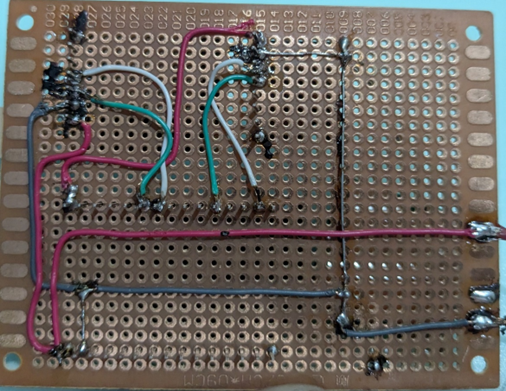
\includegraphics[width=0.8\textwidth]{figures/3_2_real_esp32_modul_1.png}
    \caption{Hình ảnh thực tế Module I đã hoàn thiện}
    \label{fig:module1_photo}
\end{figure}

Sơ đồ nguyên lý chi tiết (schematic) của Module I được vẽ bằng phần mềm KiCad và được đính kèm trong \textbf{Phụ lục B}.

\subsubsection{Module II: Camera giám sát}
\label{ssec:module_two}

Module này đóng vai trò xác nhận sự kiện té ngã bằng hình ảnh. Nó được đặt ở các khu vực giám sát trọng yếu như phòng khách sảnh hoặc phòng sinh hoạt chung. Các thành phần chính bao gồm:

\begin{figure}[H]
    \centering
    \includegraphics[width=0.8\textwidth]{figures/3_2_esp32_modul_1.pdf}
    \caption{Hình ảnh thực tế Module II}
    \label{fig:module2_photo}
\end{figure}

* \textbf{Bộ vi điều khiển ESP32-S3-N16R8}: Được lựa chọn do có bộ xử lý mạnh mẽ hơn và dung lượng bộ nhớ lớn hơn (16MB Flash và 8MB PSRAM), cần thiết để xử lý luồng dữ liệu hình ảnh nặng từ camera.
* \textbf{Module camera OV5640}: Đây là một cảm biến camera 5MP có khả năng chụp ảnh và quay video chất lượng cao. Module này thu thập luồng video liên tục và gửi đến máy chủ để phân tích bằng Python, giúp xác nhận sự kiện té ngã và giảm thiểu các cảnh báo sai.

\subsubsection{Bảng tổng hợp các thành phần phần cứng}
\label{ssec:component_summary}

Bảng \ref{tab:hardware_components} dưới đây tóm tắt các thành phần chính của hai module, cùng với vai trò cụ thể của chúng trong hệ thống.

\begin{table}[H]
    \centering
    \caption{Tổng hợp các thành phần phần cứng}
    \label{tab:hardware_components}
    \begin{tabular}{|l|l|l|l|}
        \hline
        \textbf{Thành phần} & \textbf{Loại Module} & \textbf{Chức năng} & \textbf{Hình ảnh} \\
        \hline
        ESP32-DevKitC-1 & Module I & Bộ vi điều khiển chính & 
\includegraphics[width=2cm]{figures/esp32.jpg} \\
        \hline
        MPU6050 & Module I & Cảm biến IMU 6 trục & 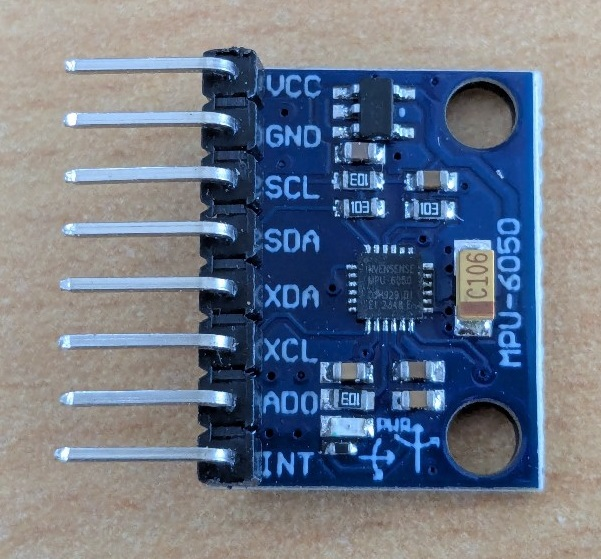
\includegraphics[width=2cm]{figures/mpu6050.jpg} \\
        \hline
        Module GPS/4G (EC800K) & Module I & Định vị và gửi tín hiệu cảnh báo & 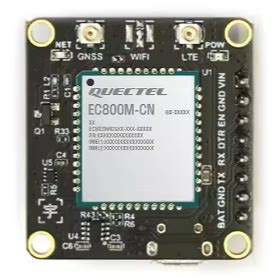
\includegraphics[width=2cm]{figures/ec800k.jpg} \\
        \hline
        Buzzer & Module I & Cảnh báo âm thanh & \includegraphics[width=2cm]{figures/buzzer.jpg} \\
        \hline
        ESP32-S3-N16R8 & Module II & Bộ vi điều khiển cho xử lý hình ảnh & \includegraphics[width=2cm]{figures/esp32_s3_n16r8.jpg} \\
        \hline
        Camera OV5640 & Module II & Cảm biến hình ảnh 5MP & \includegraphics[width=2cm]{figures/ov5640.jpg} \\
        \hline
    \end{tabular}
\end{table}
